\pdfminorversion=4
\documentclass[aspectratio=169]{beamer}

\mode<presentation>
{
  \usetheme{default}
  \usecolortheme{default}
  \usefonttheme{default}
  \setbeamertemplate{navigation symbols}{}
  \setbeamertemplate{caption}[numbered]
  \setbeamertemplate{footline}[frame number]  % or "page number"
  \setbeamercolor{frametitle}{fg=white}
  \setbeamercolor{footline}{fg=black}
} 

\usepackage[english]{babel}
\usepackage{inputenc}
\usepackage{tikz}
\usepackage{courier}
\usepackage{array}
\usepackage{bold-extra}
\usepackage{minted}
\usepackage[thicklines]{cancel}
\usepackage{fancyvrb}

\xdefinecolor{dianablue}{rgb}{0.18,0.24,0.31}
\xdefinecolor{darkblue}{rgb}{0.1,0.1,0.7}
\xdefinecolor{darkgreen}{rgb}{0,0.5,0}
\xdefinecolor{darkgrey}{rgb}{0.35,0.35,0.35}
\xdefinecolor{darkorange}{rgb}{0.8,0.5,0}
\xdefinecolor{darkred}{rgb}{0.7,0,0}
\definecolor{darkgreen}{rgb}{0,0.6,0}
\definecolor{mauve}{rgb}{0.58,0,0.82}

\title[2024-10-21-chep2024-hep-help]{\vspace{0.5 cm} \\ HEP-Help: a first-stop helpline for particle physics software \\ \vspace{-0.75 cm}\hspace{7 cm}\uncover<2->{
\includegraphics[height=2 cm]{PLOTS/in-progress.png}}\vspace{-1.75 cm}}
\author{Jim Pivarski}
\institute{Princeton University -- IRIS-HEP}
\date{October 21, 2024}

\usetikzlibrary{shapes.callouts}

\begin{document}

\logo{\pgfputat{\pgfxy(0.11, 7.4)}{\pgfbox[right,base]{\tikz{\filldraw[fill=dianablue, draw=none] (0 cm, 0 cm) rectangle (50 cm, 1 cm);}\mbox{\hspace{-8 cm}
\includegraphics[height=1 cm]{princeton-logo-long.png}\hspace{0.1 cm}\raisebox{0.1 cm}{
\includegraphics[height=0.8 cm]{iris-hep-logo-long.png}}\hspace{0.1 cm}}}}}

\begin{frame}
  \titlepage
\end{frame}

\logo{\pgfputat{\pgfxy(0.11, 7.4)}{\pgfbox[right,base]{\tikz{\filldraw[fill=dianablue, draw=none] (0 cm, 0 cm) rectangle (50 cm, 1 cm);}\mbox{\hspace{-8 cm}
\includegraphics[height=1 cm]{princeton-logo.png}\hspace{0.1 cm}\raisebox{0.1 cm}{
\includegraphics[height=0.8 cm]{iris-hep-logo.png}}\hspace{0.1 cm}}}}}

% Uncomment these lines for an automatically generated outline.
%\begin{frame}{Outline}
%  \tableofcontents
%\end{frame}

% START START START START START START START START START START START START START

\begin{frame}{For a long time, I've wanted a ``StackOverflow for HEP''}
\large
\vspace{0.5 cm}
\begin{columns}[t]
\column{0.33\linewidth}
\textcolor{darkblue}{PyHEP 2019:} I tried to get everybody to {\it use} StackOverflow, with tags to carve out our space within it.

\vspace{0.25 cm}
\fbox{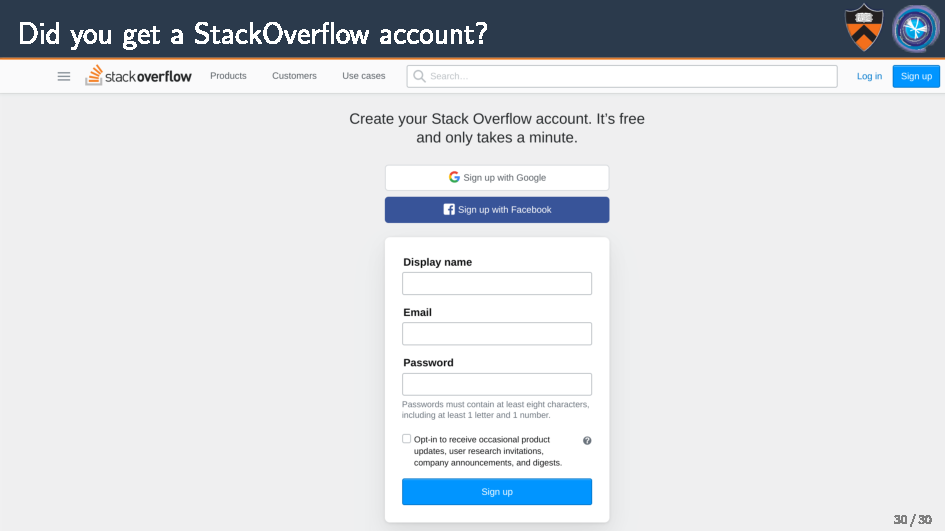
\includegraphics[width=\linewidth]{PLOTS/2019_10_17_pyhep_awkward-slide.pdf}}

%% \small
%% \vspace{0.25 cm}
%% \uncover<2->{\textcolor{gray}{(Creating our own StackExchange site would be a bigger community effort.)}}

\column{0.33\linewidth}
\uncover<2->{\textcolor{darkblue}{JLab Future Trends 2022:} I acknowledged that it's not going well.}

\vspace{0.25 cm}
\uncover<2->{\fbox{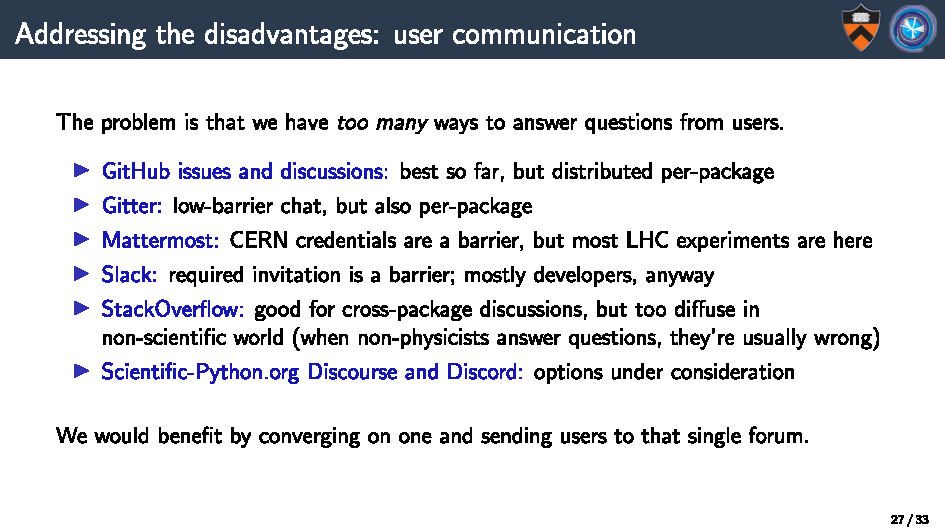
\includegraphics[width=\linewidth]{PLOTS/2022_09_28_future_trends_python-slide.pdf}}}

%% \small
%% \vspace{0.25 cm}
%% \uncover<4->{\textcolor{gray}{(Despite the tags, StackOverflow questions get more answers from general programmers who don't recognize the need for scaling.)}}

\column{0.33\linewidth}
\uncover<3->{\textcolor{darkblue}{Analysis Ecosystem II 2022} and \textcolor{darkblue}{PyHEP.dev 2023:} Brainstorming sessions, never landed on a solution.}

\vspace{0.25 cm}
\uncover<3->{\fbox{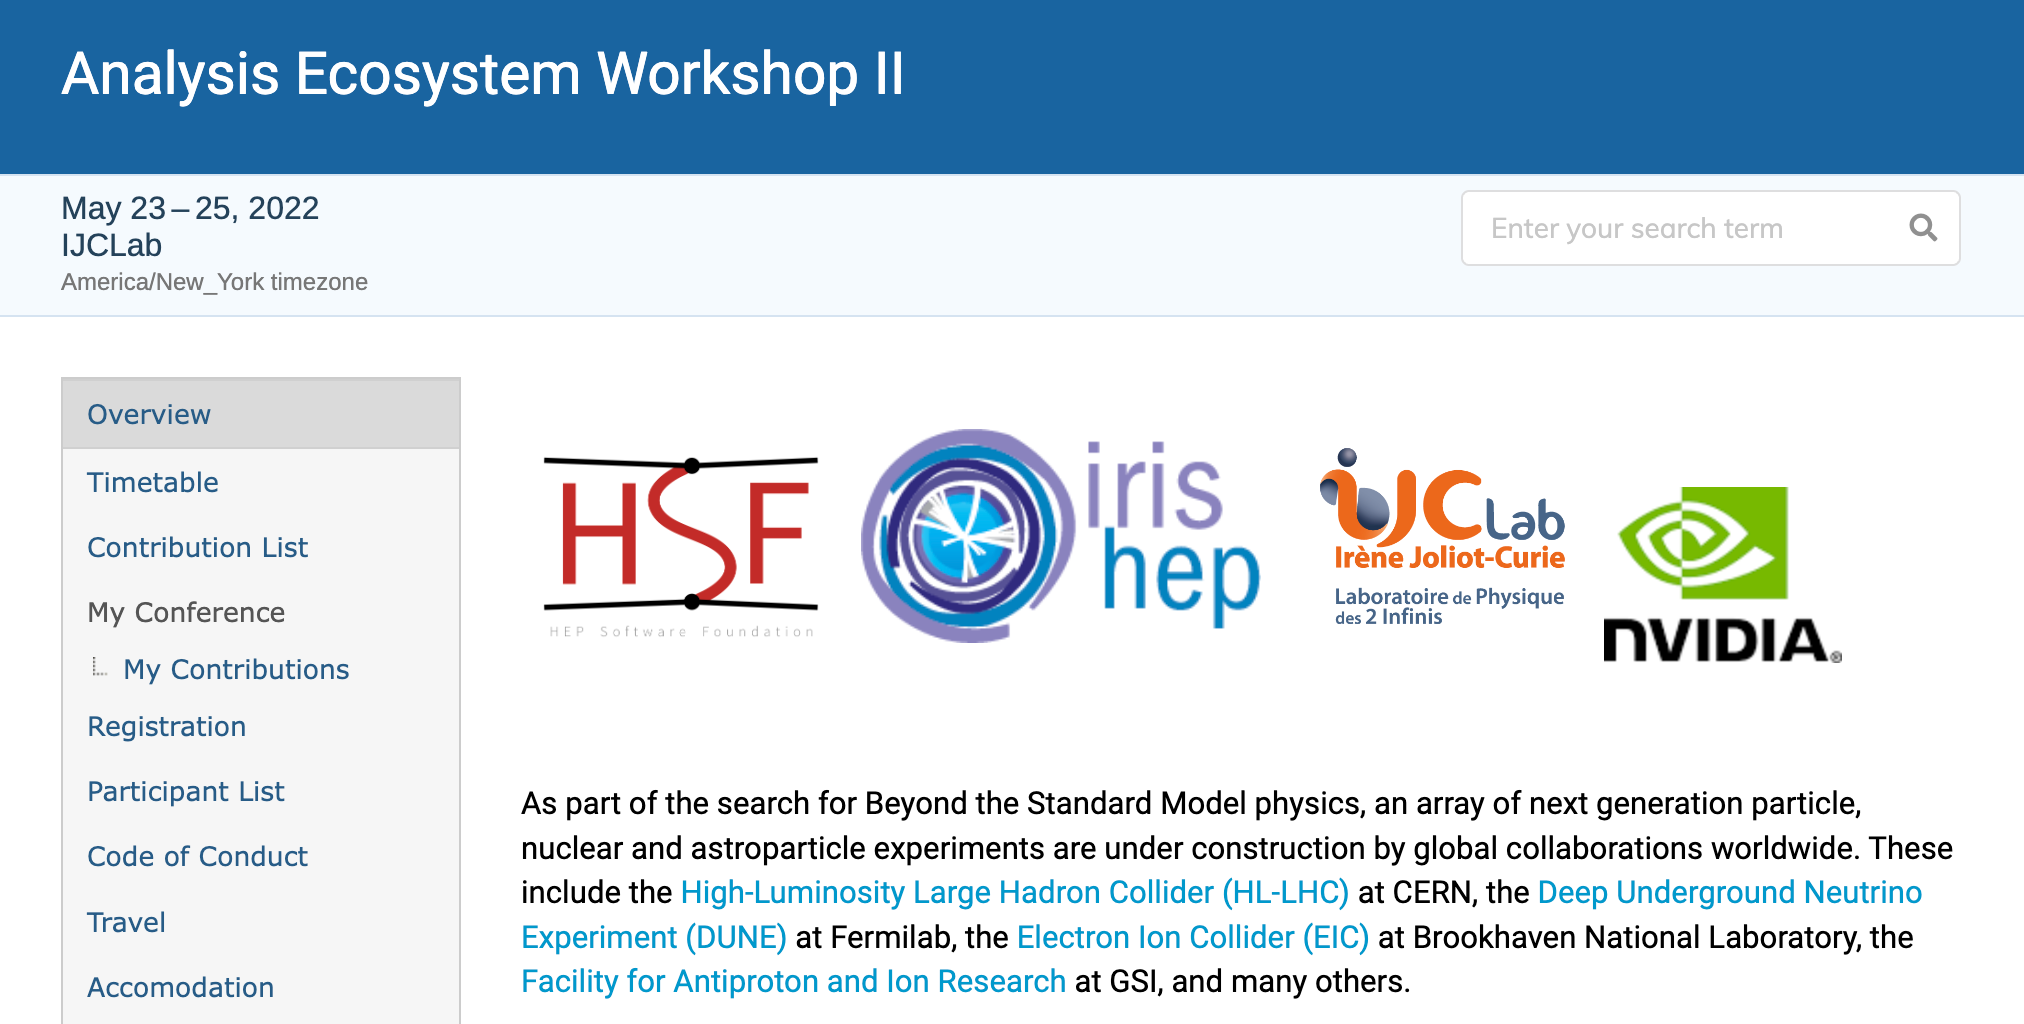
\includegraphics[width=\linewidth]{PLOTS/2022-05-23-analysis-ecosystem-ii-banner.png}}}

\vspace{0.25 cm}
\uncover<3->{\fbox{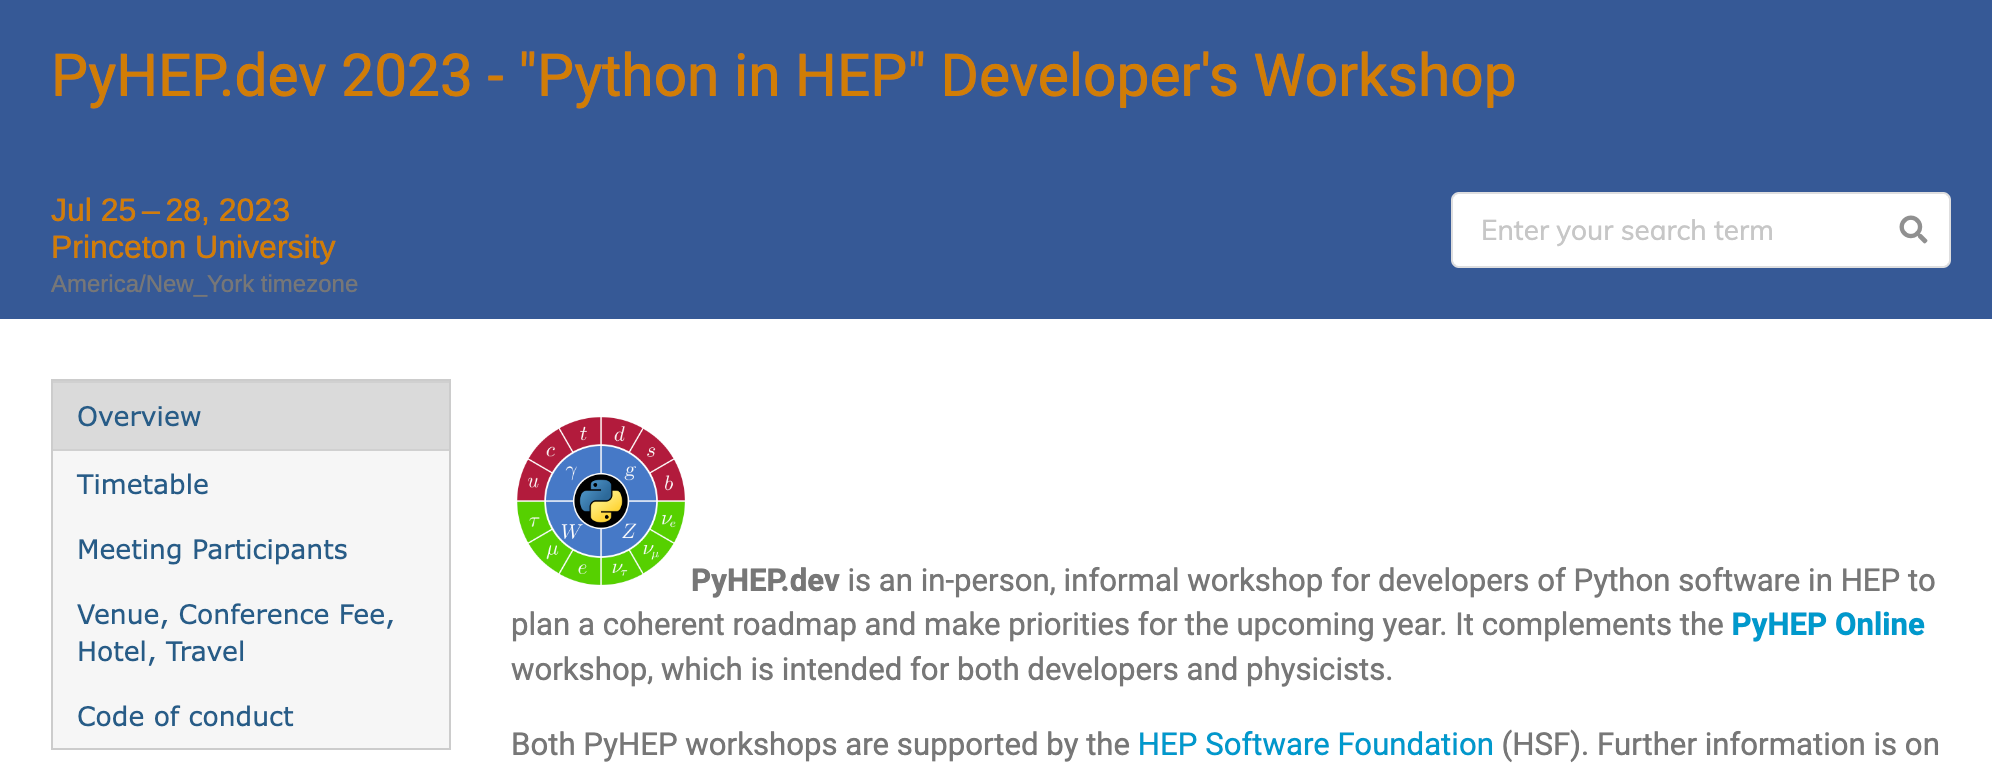
\includegraphics[width=\linewidth]{PLOTS/2023-07-25-pyhepdev-banner.png}}}

\end{columns}
\end{frame}

\begin{frame}{The current state of user-help across HEP software packages}
\vspace{0.25 cm}
\begin{center}
\fbox{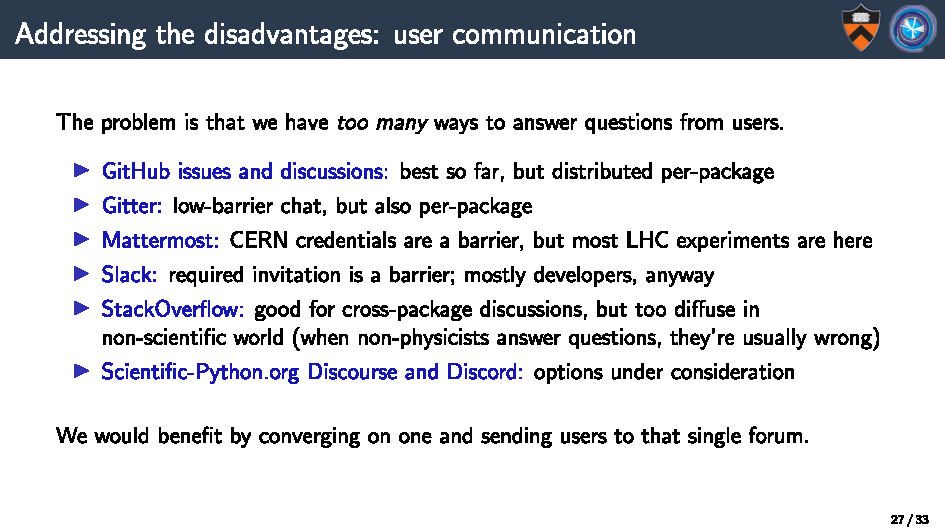
\includegraphics[width=0.9\linewidth]{PLOTS/2022_09_28_future_trends_python-slide.pdf}}
\end{center}
\end{frame}

\begin{frame}{The ROOT Forum does not have this problem}
\large
\vspace{0.25 cm}

\begin{center}
\fbox{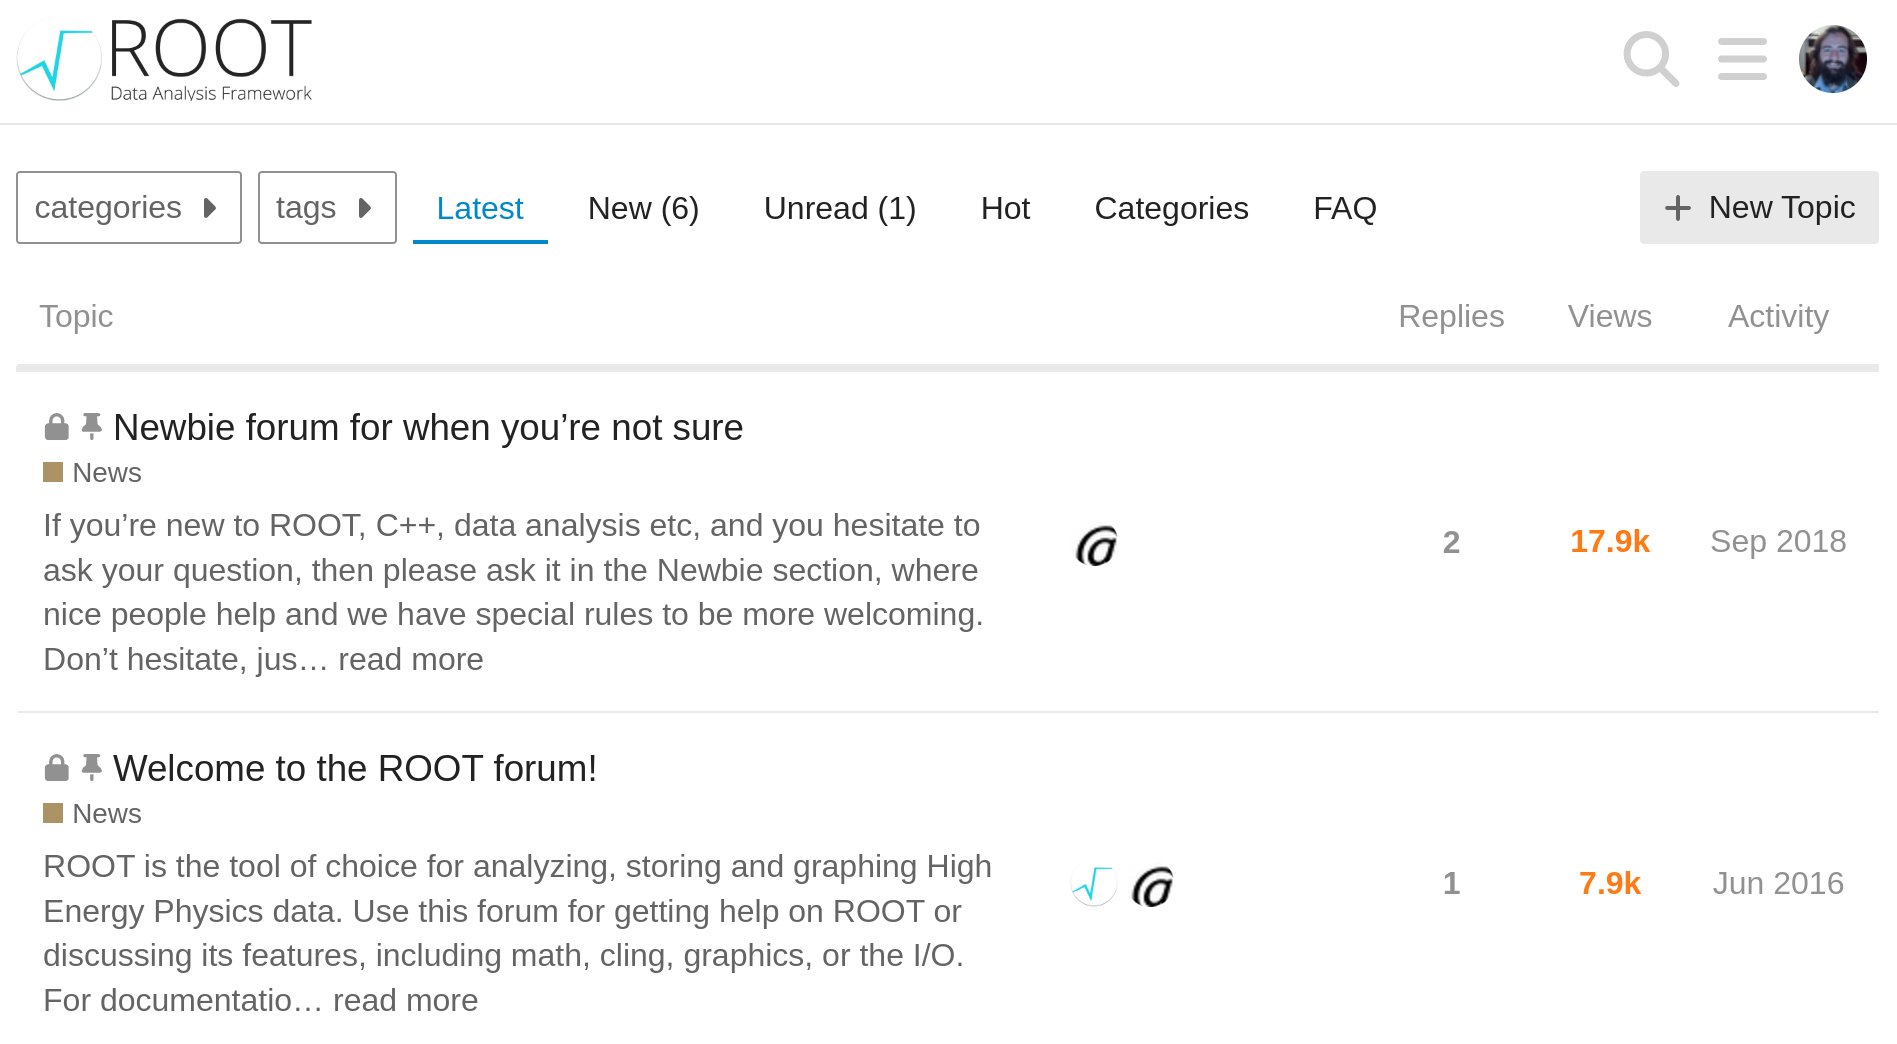
\includegraphics[width=0.7\linewidth]{PLOTS/root-forum-banner.png}}
\end{center}

\begin{itemize}
\item<2-> It's easy for newcomers to find, and ROOT team ensures that there's always someone ``on shift'' to answer questions.
\item<3-> Deep historical archive of past questions and answers.
\end{itemize}
\end{frame}

\begin{frame}{\mbox{ }}
\large
\vspace{0.5 cm}
Similarly, IRIS-HEP Slack, Coffea Users in CMS Mattermost, and some GitHub Discussions are very active.

\vspace{1 cm}
\uncover<2->{Moving active communities is hard, and runs the risk of dispersing them instead.}

\vspace{1 cm}
\begin{uncoverenv}<3->
\textcolor{darkblue}{Better strategy:} make an entry point that

\vspace{0.25 cm}
\begin{itemize}
\item shows people where a question has already been answered
\item leads people to the right place to engage with already-active communities.
\end{itemize}
\end{uncoverenv}
\end{frame}

\begin{frame}{New monkey wrench}
\vspace{0.17 cm}
\begin{columns}
\column{1.15\linewidth}
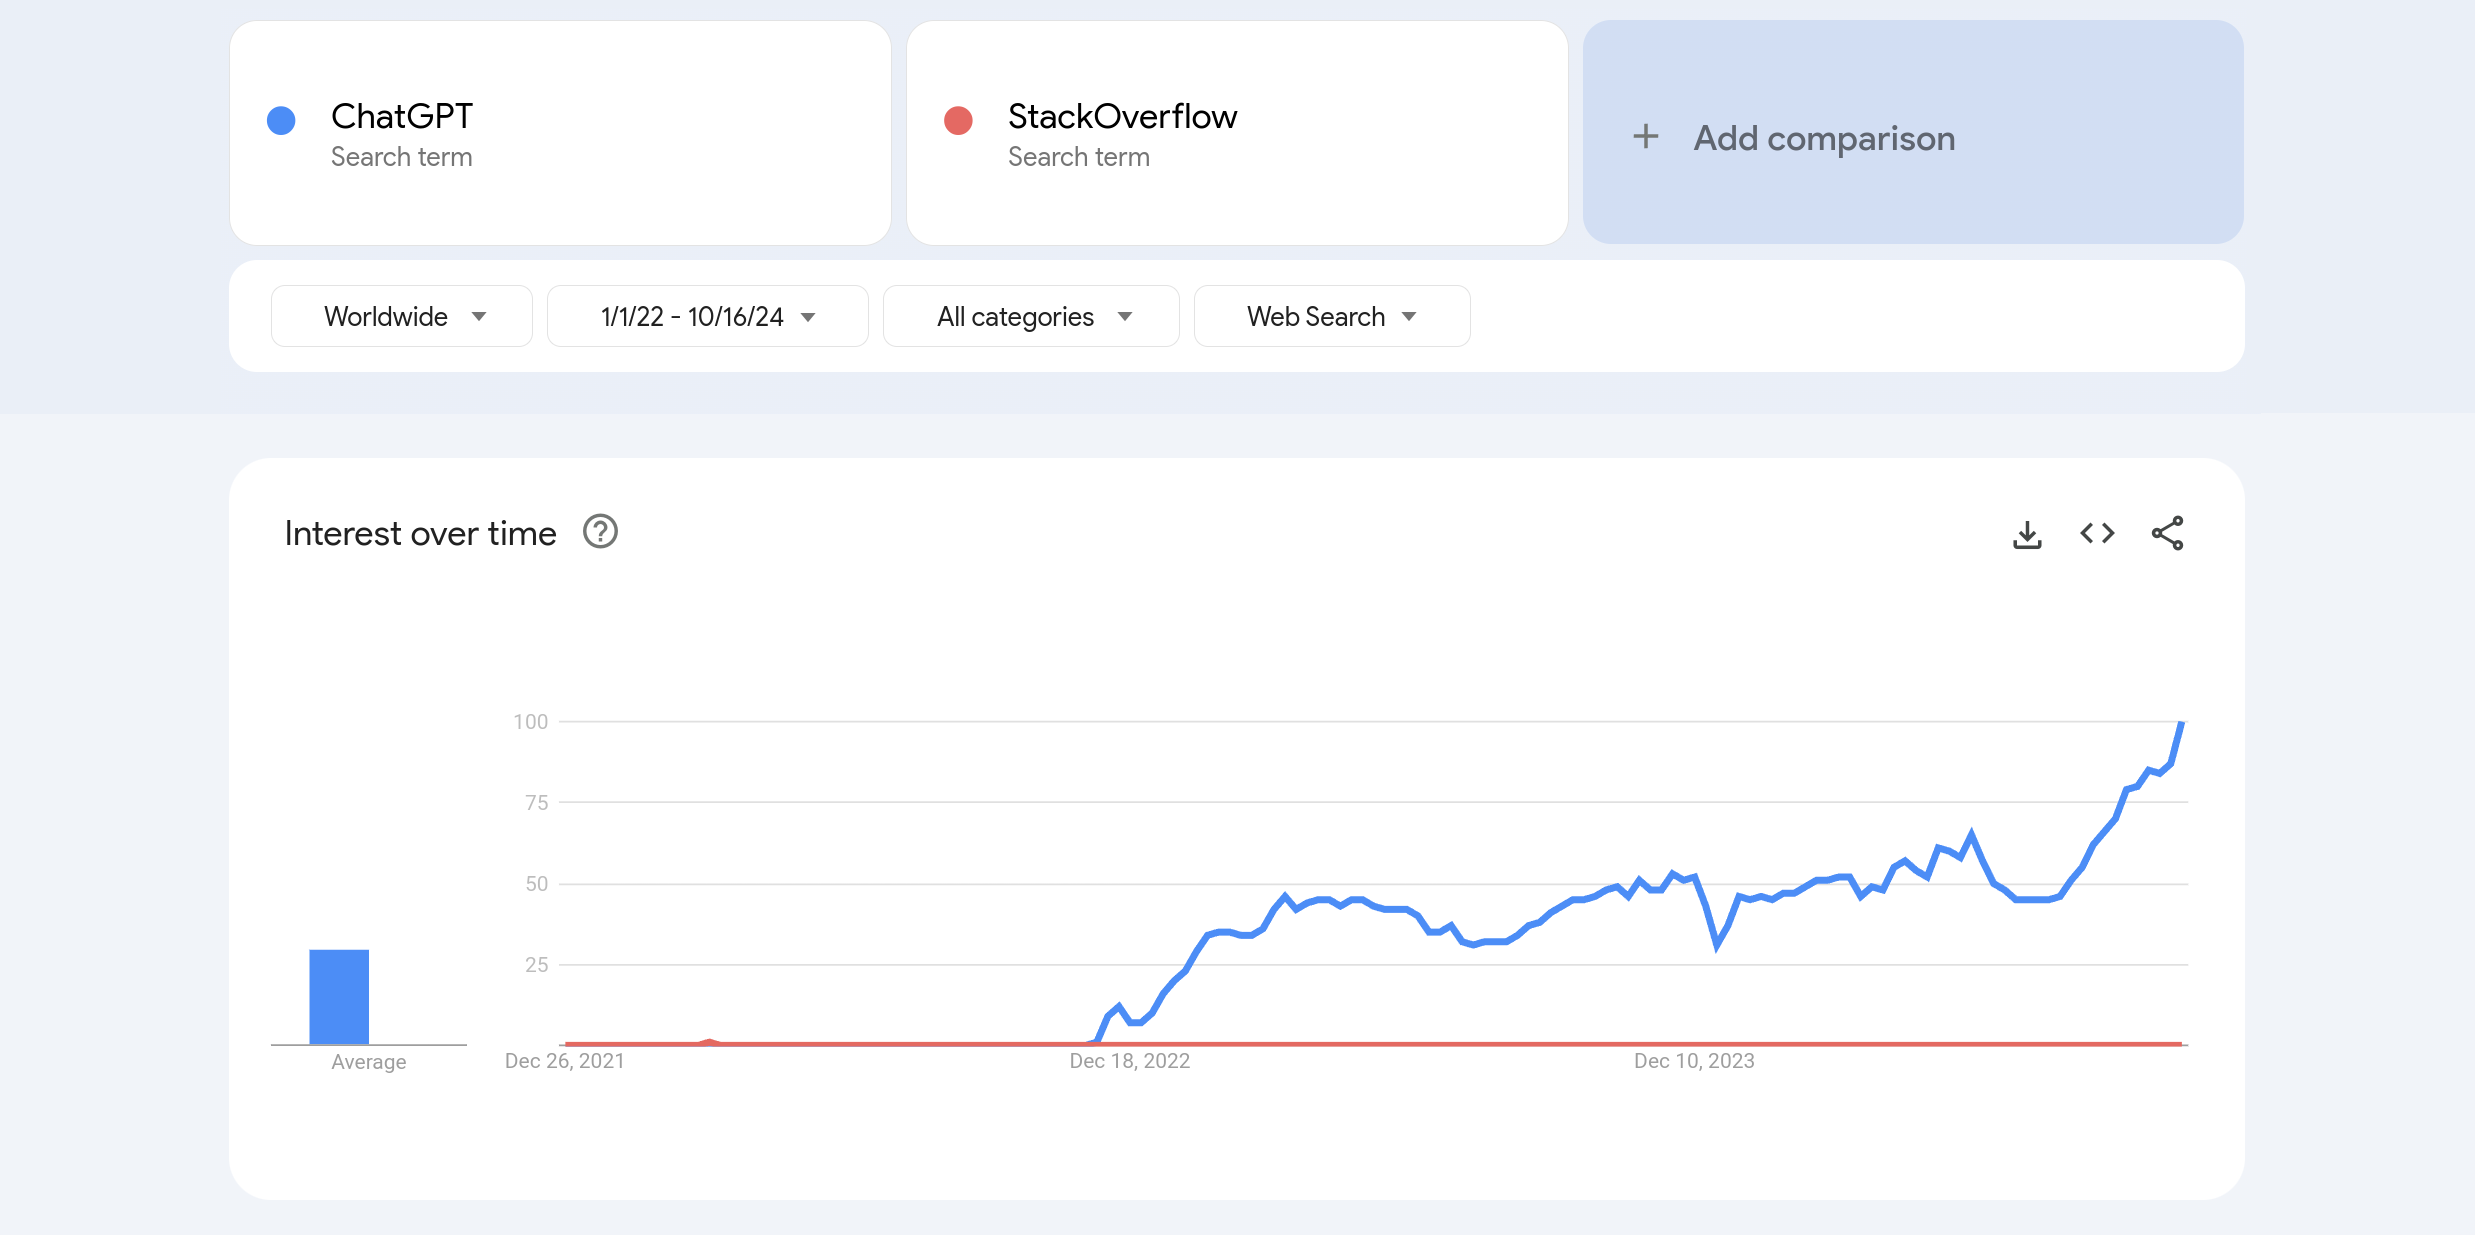
\includegraphics[width=\linewidth]{PLOTS/googletrends-chatgpt.png}
\end{columns}
\end{frame}

\begin{frame}{\mbox{ }}
\Large
\vspace{1 cm}

Can a Large Language Model (LLM) be a first responder, either to answer questions or to send people to a forum where their can be answered or has already been answered?

\vspace{0.5 cm}
\begin{center}
\uncover<2->{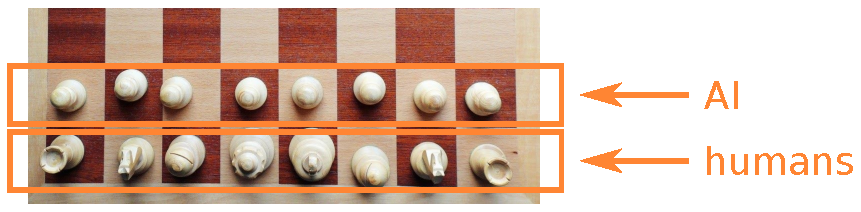
\includegraphics[width=0.8\linewidth]{PLOTS/ai-humans-chess-metaphor.pdf}}
\end{center}
\end{frame}



\end{document}
